\documentclass[hidelinks,11pt]{article}
\usepackage{setspace}
\usepackage{mathpazo}
\usepackage[makeroom]{cancel}
\usepackage{arabtex}
\usepackage{indentfirst}
\usepackage[md]{titlesec}
\usepackage{xcolor}
\usepackage{mwe}
\usepackage{amsmath}
\usepackage{lipsum}
\usepackage{graphicx}
\usepackage{tikz}
\usepackage[makeroom]{cancel}
\usetikzlibrary{positioning}
\usepackage{subcaption}
\usepackage{caption}
\usepackage{rotating}
\usepackage[margin=1.2in]{geometry}
\usepackage{graphicx}
\usepackage[authoryear]{natbib}
\usepackage[pagebackref=true]{hyperref}
\hypersetup{citecolor=blue}
\usepackage{arabtex}
\usepackage{amssymb}
\usepackage{fancyhdr}
\begin{document}
\bibliographystyle{apsa-leeper}
\setarab
\vocalize
\transtrue
\arabfalse
\title{Diagnosing the violation of assumptions when estimating OLS regressions to recover average causal effects under unconfoundedness: \\A review of new tools}
      \maketitle
\doublespacing


\pagestyle{fancy}
\fancyhf{}
\rhead{Code\# 288 \\ Methods 2nd Field \\ Page \thepage}
\rfoot{Page \thepage of 25}

\begin{abstract}
I discuss recently developed tools for evaluating OLS estimates of average causal effects under unconfoundedness. The first tool, regression weights introduced by \citet{aronowsamii2016}, helps analysts diagnose heterogeneity that may be biasing estimates. The second tool, a sensitivity analysis introduced by \citet{cinellihazlett2020}, helps analysts understand the severity of unmeasured confounding necessary to alter substantive conclusions. I walk through the logic of each tool, using simple simulations and a replication study to illustrate threats to inference and how the tools can diagnose them.

\end{abstract}

\section{Introduction}

A large body of research in political science uses ordinary least squares (OLS) regression to estimate average causal effects under the identification assumption of unconfoundedness. As is exhaustively covered in textbook treatments, the validity of inferences made using this combination of estimand, identification strategy, and estimator requires that several assumptions are met. Two assumptions that are frequently used to derive the desirable properties of regression estimates in this context are unconfoundedness, or conditional independence, and effect homogeneity. The first requires that the observed treatment values in the population are independent from the potential outcomes under treatment and control conditional on covariates. The second requires that the effect of treatment is the same for all units.

Both assumptions may be difficult to justify in some settings. Yet it is often unclear what the consequences of minor violations are. When is violation of these assumptions likely to change our substantive conclusions? The purpose of this essay is to review recently developed tools that help answer this question. Throughout, I use simple simulation examples to illustrate threats to inference and to explore the limits of these tools. I also replicate an existing study in the section on sensitivity analysis.

I first address the assumption of homogeneity. After a discussion of the most severe case of heterogeneity---when treatment effects vary across treatment and control groups, violating the unconfoundedness assumption---I review the less severe case when the unconfoundedness assumption is met. In this context, I discuss the multiple-regression weights introduced by \citet{aronowsamii2016}. The purpose of these weights is to estimate how regression estimates weigh individual causal effects in the population of units. When the weights on some units are bigger than others, regression estimates no longer recover the average causal effect of interest; instead, analysts must make do with a weighted average of individual causal effects---a quantity unlikely to be of substantive interest.

I then address the assumption of unconfoundedness and review the sensitivity analysis introduced by \citet{cinellihazlett2020}. Their procedure allows analysts to judge how severe total unmeasured confounding would have to be to overturn substantive results.

\section{Recovering causal effects under selection on observables}

Researchers who estimate average causal effects under unconfoundedness using OLS are choosing a combination of estimand, identification strategy based on a causal model, and estimator, even if these choices are sometimes not made explicit. Below, I pin down some notation and review the standard results that justify this combination.

\subsection{Preliminaries and notation}

We are interested in the average causal effect of some treatment $D$ on some outcome $Y$. For simplicity, we assume that the treatment is binary such that $D \in \{0,1\}$.\footnote{Although the tools we will be reviewing also work for multi-valued treatments} We can use the notion of potential outcomes to define this causal effect in terms simple of counterfactuals. For each individual $i$ in a population of interest, we can imagine the outcome $Y_i$ taking on different values when they receive different treatments. Write the potential outcome that we would observe for individual $i$ if they were treated as $Y_i(1)$, and the potential outcome if not treated as $Y_i(0)$. For each unit, there are two potential outcomes but only one observed potential outcome: $Y_i = D_i Y_i(1) + (1-D_i)Y_i(0)$.

The average causal effect averages over the difference between potential outcomes under treatment and control for each unit. This is our estimand.

$$\bar \tau = \mathbb{E}[Y_i(1)]-\mathbb{E}[Y_i(0)]$$

\subsection{Identification}

The average causal effect is \emph{causally identified} under several standard assumptions, which we will assume are met. The first assumption, overlap, entails that the probability of receiving any level of the treatment is greater than zero and less than one. The second, SUTVA (stable unit value treatment assumption), entails that potential outcomes in the population are all defined with respect to the same treatment, $D$, and that there is no interference between units. The final assumption, conditional independence, requires that potential outcomes are independent of realized treatment assignment conditional on some vector of covariates $\boldsymbol{X}$.

$$(Y_i(1),Y_i(0)) \perp D_i | \boldsymbol{X_i}$$

Under these assumptions, our average causal effect is point identified: it can be written as a function of observable variables, making it \emph{possible} to asymptotically estimate the actual causal effect. We can re-write the causal effect as $\mathbb{E}[Y_i|D_i=1,\boldsymbol{X_i}]-\mathbb{E}[Y_i|D_i=0,\boldsymbol{X_i}]$, which is a conditional expectation function that can be estimated from observed data.

\subsection{Estimation via OLS}

At this point, textbook treatments point out that a simple regression is the best (in the sense of minimizing mean-squared error) linear approximation of this underlying conditional expectation function \citep{angristpischke2008}. Having justified the previous assumptions -- those necessary to give the conditional expectation function a causal interpretation -- researchers often move to estimating a version of the following equation using ordinary least squares (OLS),

$$Y_i = \beta_0 + \beta_1 D_i + \boldsymbol{X_i} \boldsymbol{\beta} + \epsilon_i$$

where $\beta_0$ is the intercept, $\beta_1$ attempts to recover an approximation of our average causal effect, $\bar \tau$, and $\epsilon_i$ is an idiosyncratic error term. This specification may also include transformations of the covariates. Often embedded in this formulation of the estimation problem is another assumption, one that is rarely made explicit in applied work. The assumption concerns effect heterogeneity. Only when the causal effect is the same for everyone do the assumptions we have made above always get us the average causal effect, or at least the best linear approximation. The important contribution of the work on heterogeneity I review is to provide guidance in how to interpret regression estimates under different assumptions about effect heterogeneity and how to diagnose when effect heterogeneity makes inferences difficult. While I first review how heterogeneity issues play out when effects are heterogeneous due to the effect of a confounder, I also show how estimates may still be biased if this is not the case.

\section{Effect heterogeneity across treatment and control groups}

\subsection{Binary treatment}

In this section, I walk through a simulated toy problem in the context of a binary treatment and outcome. The design of the simulation is meant to emulate a more realistic setting where the unconfoundedness assumption is still met. The goal is to show how, even after adjusting for baseline differences, effect heterogeneity between units with different treatment statuses bias estimates.

Covariates in the simulation act as confounders in two ways. First, one set of covariates affects both selection into treatment via the propensity scores as well as baseline potential outcomes. A second set of covariates affects selection as well as the size of individual treatment effects. The simulation is meant to emulate the set-up in \citet{kangshafer2007}, by making it likely that any models specified by researchers are slightly, but not grossly misspecified.

First I sample the covariates from a multivariate normal distribution with the identity matrix as the variance-covariance matrix. The propensity scores are generated from the model

$$e_i = expit(-z_{i1} - 2z_{i2} - 3z_{i3} - \epsilon_i) \;\;\;\;\;\;\;\;\; where\;\;\; \epsilon \sim \mathcal{N}(0,1)$$

the baseline potential outcomes from the model

$$Y_i(0) = 2z_{i1} + 3z_{i2} + \eta_i \;\;\;\;\;\;\;\; where\;\;\; \eta \sim \mathcal{N}(15,4)$$

and the treatment effects from the model

$$\tau_i = 2z_{i2} + z_{i3} + \xi_i\;\;\;\;\;\;\;\;\text{where} \;\;\;\ xi_i  \sim \mathcal{N}(1,2)\;\;$$

In this setting, a logistic regression of treatment on the covariates would be the correct model for the propensity score $e$; a linear regression would be the same for the outcomes. But, following \citet{kangshafer2007}, we only observe transformed or coarsened versions of the covariates used in the true data-generating process:

$$x_1 = exp(z_1 / 2)$$
$$x_2 = z_2 / (1 + exp(z_1)) + 10$$
$$x_3 = roundInt(5z_3) + 5$$

For the last covariate, $roundInt$ rounds to the nearest integer. The functional forms necessary to correctly specify the model are now less likely to be gleaned from the data, and models for the propensity score and outcome likely to be at least slightly misspecified.

\subsection{Effect heterogeneity between treatment and control groups}

\begin{figure}
  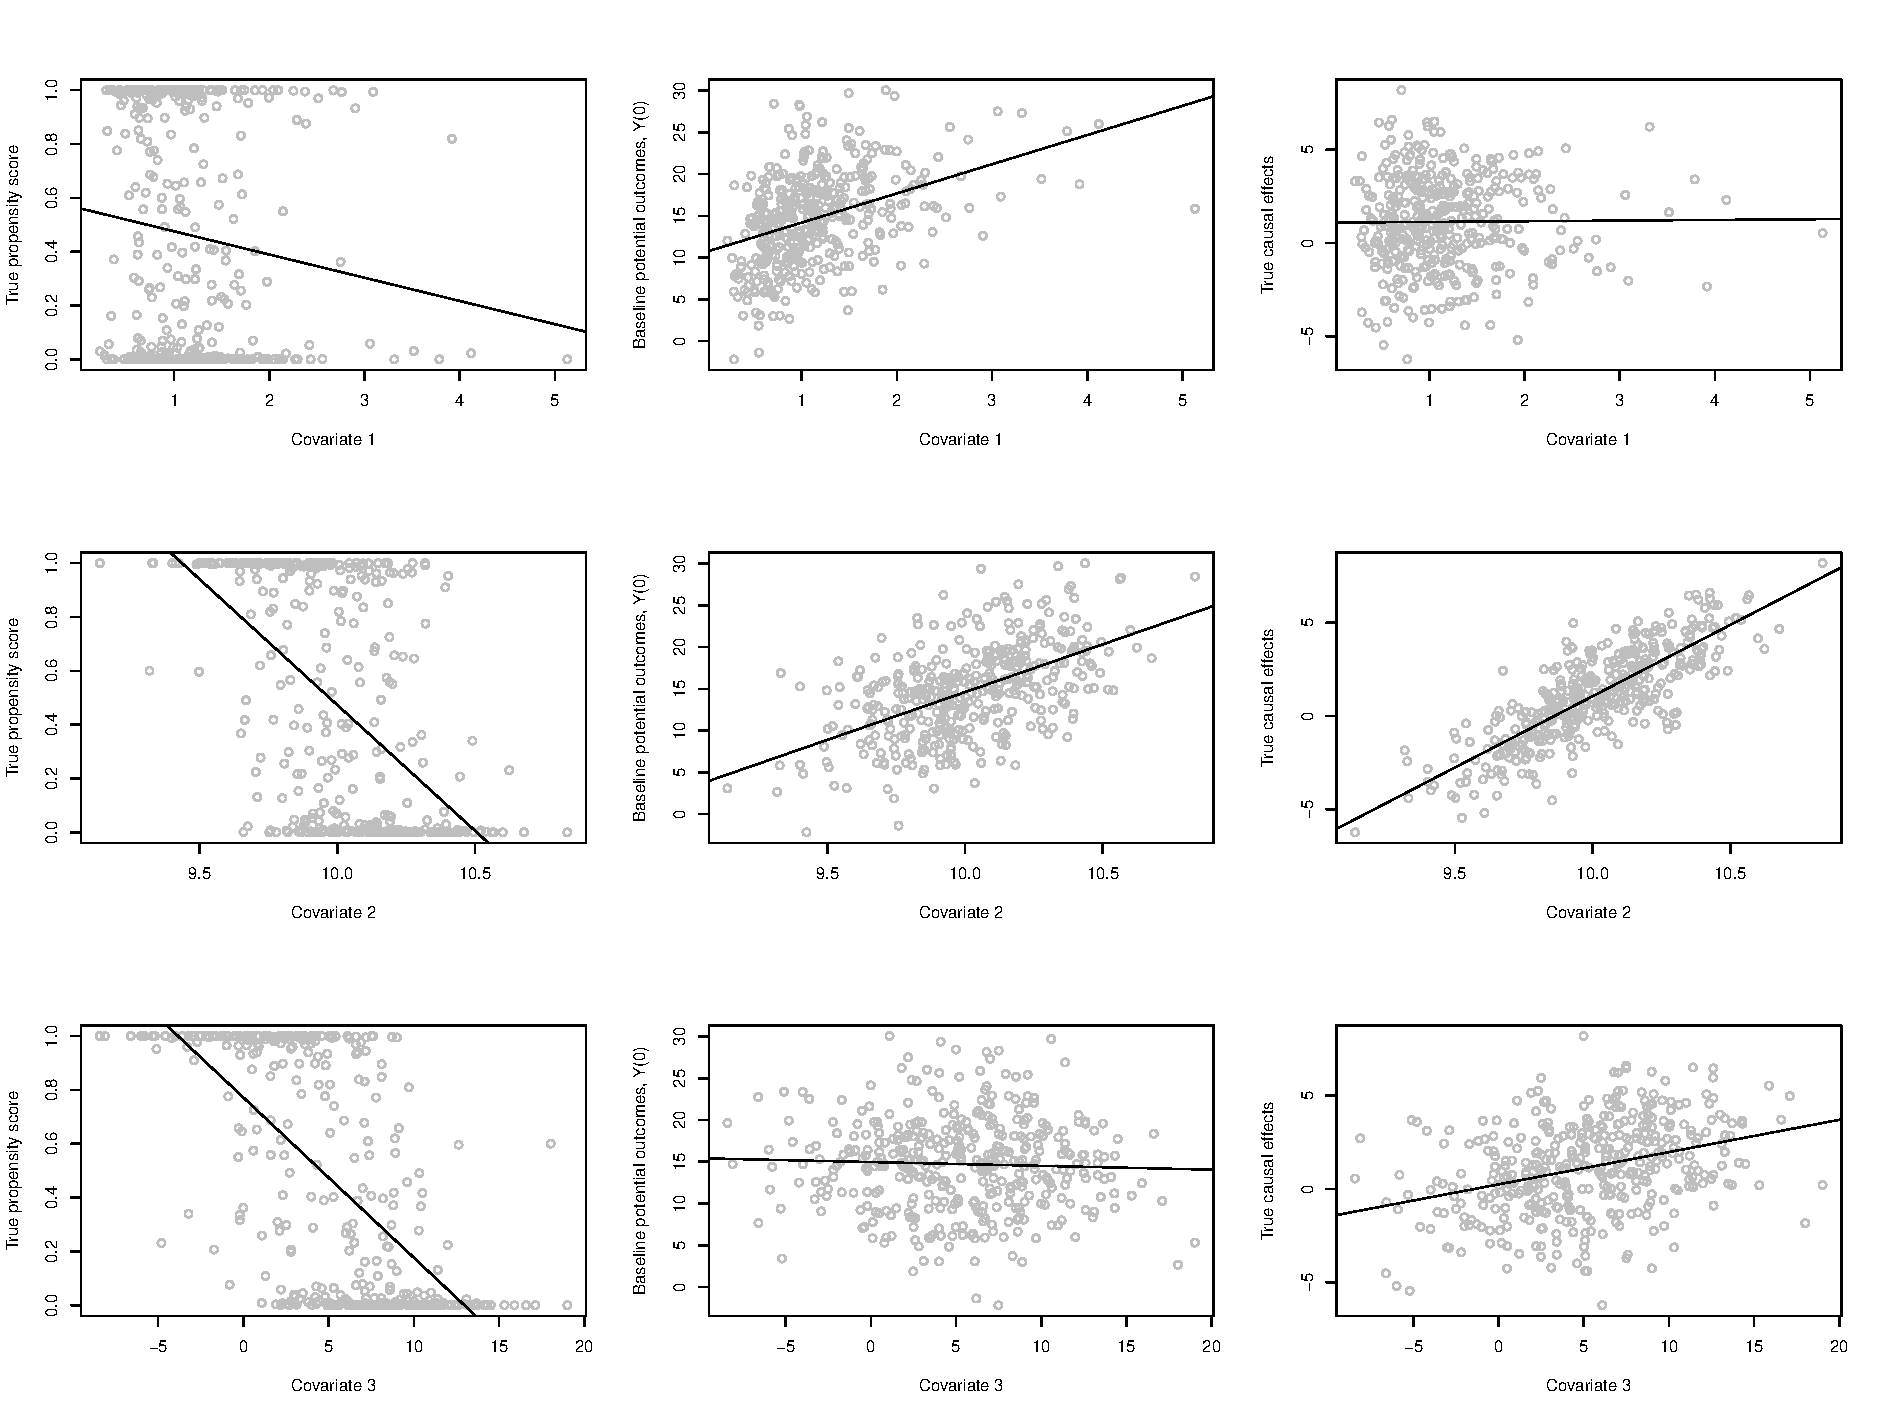
\includegraphics[width=\linewidth]{../plots/selection.pdf}
  \caption{\emph{The panels use data from one of the simulated samples to show the selection problems and heterogeneous treatment effects in the data-generating process. In each row, the true propensity score and baseline potential outcomes under control are plotted against values of a different covariate. In this data-generating process, the probability of receiving treatment is smaller for units with larger values of the covariates as shown by the panels on the left. At the same time, potential outcomes under control are greater for units with larger values of the covariates as shown by panels on the right. The result is that simple comparisons of outcomes across treatment groups will underestimate true average causal effects. The observed outcomes in the control group will not approximate outcomes we would have observed for treated units if they had been assigned to control; instead, realized potential outcomes under control of units that actually end up in control (those with low propensity scores) will end up being greater than the potential outcomes under control for treated units. The same problem obtains for treatment effects: treatment effects are larger for covariate values with lower propensity scores.}}
  \label{selection}
\end{figure}


In our setting, the true average treatment effect is positive and the estimate returned by a naive regression of outcome on treatment is biased downward. In this case, part of the bias is due to effect heterogeneity. Treatment effects are smaller for units with covariate values that cause them to select into treatment. Figure \ref{selection} illustrates this issue. The panels on the left of the figure plot the true propensity scores used to generate treatment against each of the covariates. Similarly, the panels on the right plot the underlying individual causal effects against the covariates. Observe that, for covariates $x_2$ and $x_3$ the units with lower covariate values have both larger propensity scores as well as smaller causal effects.


To see how data-generating processes that produce effect heterogeneity across treatment and control groups bias inferences, consider the following decomposition \citep{morganwinship1999}:


$$\overbrace{(\overline{Y_i(1)|D_i=1} - \overline{Y_i(0)|D_i=0}}^{\text{Naive estimator}}) = $$

$$\underbrace{\bar \tau}_{ACE}  + \underbrace{\{(\overline{Y_i(0)|D_i=1}) - (\overline{Y_i(0)|D_i=0})\}}_{\text{Baseline differences}} + (1 - \pi)\underbrace{\{(\overline{\tau_i|D_i=1}) - (\overline{\tau_i|D_i=0})\}}_{\text{Heterogeneous effects}}$$

where $\pi$ denotes the proportion of units treated. In the absence of controls, the ``naive'' regression recovers the true causal (term one) effect plus the difference in potential outcomes under control (term two) plus a weighted difference in average treatment effects between treated and control units (term three). The weight is the proportion of untreated units. For the data in the toy example, the decomposition plays out as follows:

$$\underbrace{-4.1}_{\text{Naive Estimator}} = \underbrace{1.1}_{\text{ACE}} + \underbrace{(-3.6)}_{\text{Baseline differences}} + \underbrace{(1 - .53)(-3)}_{\text{Heterogeneous effects}}$$

Adjusting for confounders of baseline differences between treatment and control groups is sufficient if there is no heterogeneity. In our example, we can see that it reduces the bias but does not eliminate it completely. If we fit the regression,\footnote{Recall that it was fairly easy to tell from the graphed data that $x_1$'s relationship with the outcome is logged.}

$$Y_i = \beta_0 + \beta_1 D_i + \beta_2 logX_{1i} + \beta_3 X_{i2} + \epsilon_i$$

we estimate a treatment effect that is, averaged over all the simulations, biased by -3.89. While still downward biased, this estimate is a significant improvement on the naive estimate whose bias is at least -7. We can achieve further improvements by also adjusting for the covariates which cause treatment effect sizes to vary across treatment and control groups. Fitting the regression

$$Y_i = \beta_0 + \beta_1 D_i + \beta_2 logX_{1i} + \beta_3 X_{i2} + \beta_4X_{i4} + \epsilon_i$$

we estimate a treatment effect with an average bias of less than .1, a further improvement. We can slightly improve on our estimates in this context, even if we introduce more flexible transformations of covariates.\footnote{In the most flexible specification, I use b-splines to transform the covariates.} Table 1 shows the results from the simulation study, showing how not controlling for covariates that induce heterogeneous treatment effects can induce serious bias.

\begin{table}[ht]
\centering
\begin{tabular}{rllrr}
  \hline
 & Estimator & Sample size & Bias & RMSE \\
  \hline
1 & No controls & n = 400 & -7.32 & 7.35 \\
  2 & Heterogeneity controls &  & -1.10 & 1.39 \\
  3 & Selection controls &  & -3.96 & 4.00 \\
  4 & Full controls &  & -0.12 & 0.80 \\
  5 & Splines &  & -0.05 & 0.77 \\
  6 & No controls & n = 1000 & -7.24 & 7.25 \\
  7 & Heterogeneity controls &  & -0.88 & 1.05 \\
  8 & Selection controls &  & -3.89 & 3.90 \\
  9 & Full controls &  & 0.09 & 0.57 \\
  10 & Splines &  & 0.06 & 0.54 \\
   \hline

\end{tabular}

\end{table}

In the next section, I review what happens when heterogeneous treatment effects do not serve as a source of confounding---and how they may nonetheless bias OLS estimates of average causal effects.

\section{Effect heterogeneity across and within treatment and control groups}

There is a difference between what our regression coefficient $\beta_1$ estimates when assuming one causal effect that is the same for everyone, and what $\beta_1$ estimates when causal effects are different for different groups of units, or different for everyone. In what follows, I review work that clarifies the implications of such effect heterogeneity for OLS estimates \citep{aronowsamii2016}. This work starts from the basic insight that when causal effects are different for different groups or individuals in the sample, OLS estimates a \emph{weighted} average of group or individual causal effects. The weights are always some function of the variance of treatment assignment.

In this section, I review the multiple regression weights introduced by \citet{aronowsamii2016}. To get their result, they impose the additional assumption that conditional expected value of treatment assignment can be expressed as a linear combination of covariates: $\mathbb{E}[D|X]$ can be written as a sum of observed $X$ weighted by a set of coefficients.

To fix some intuition, consider the following thought experiment, illustrated with simulated data in Figure \ref{fig_1_a}. The simulations are fairly standard in that the covariate, treatment, and outcome, are normally distributed; treatment and outcome are confounded in that both are linear combinations of the covariate. We are in the same setting, estimating the causal effect of a continuous $D$ on $Y$; all the assumptions we have made so far hold, allowing us to achieve causal identification by conditioning on $X$. The only twist is that treatment effects are different for every individual. Instead of one causal effect $\tau$ for everyone, every individual has a causal effect $\tau_i$ that may differ across individuals.

\begin{figure}
  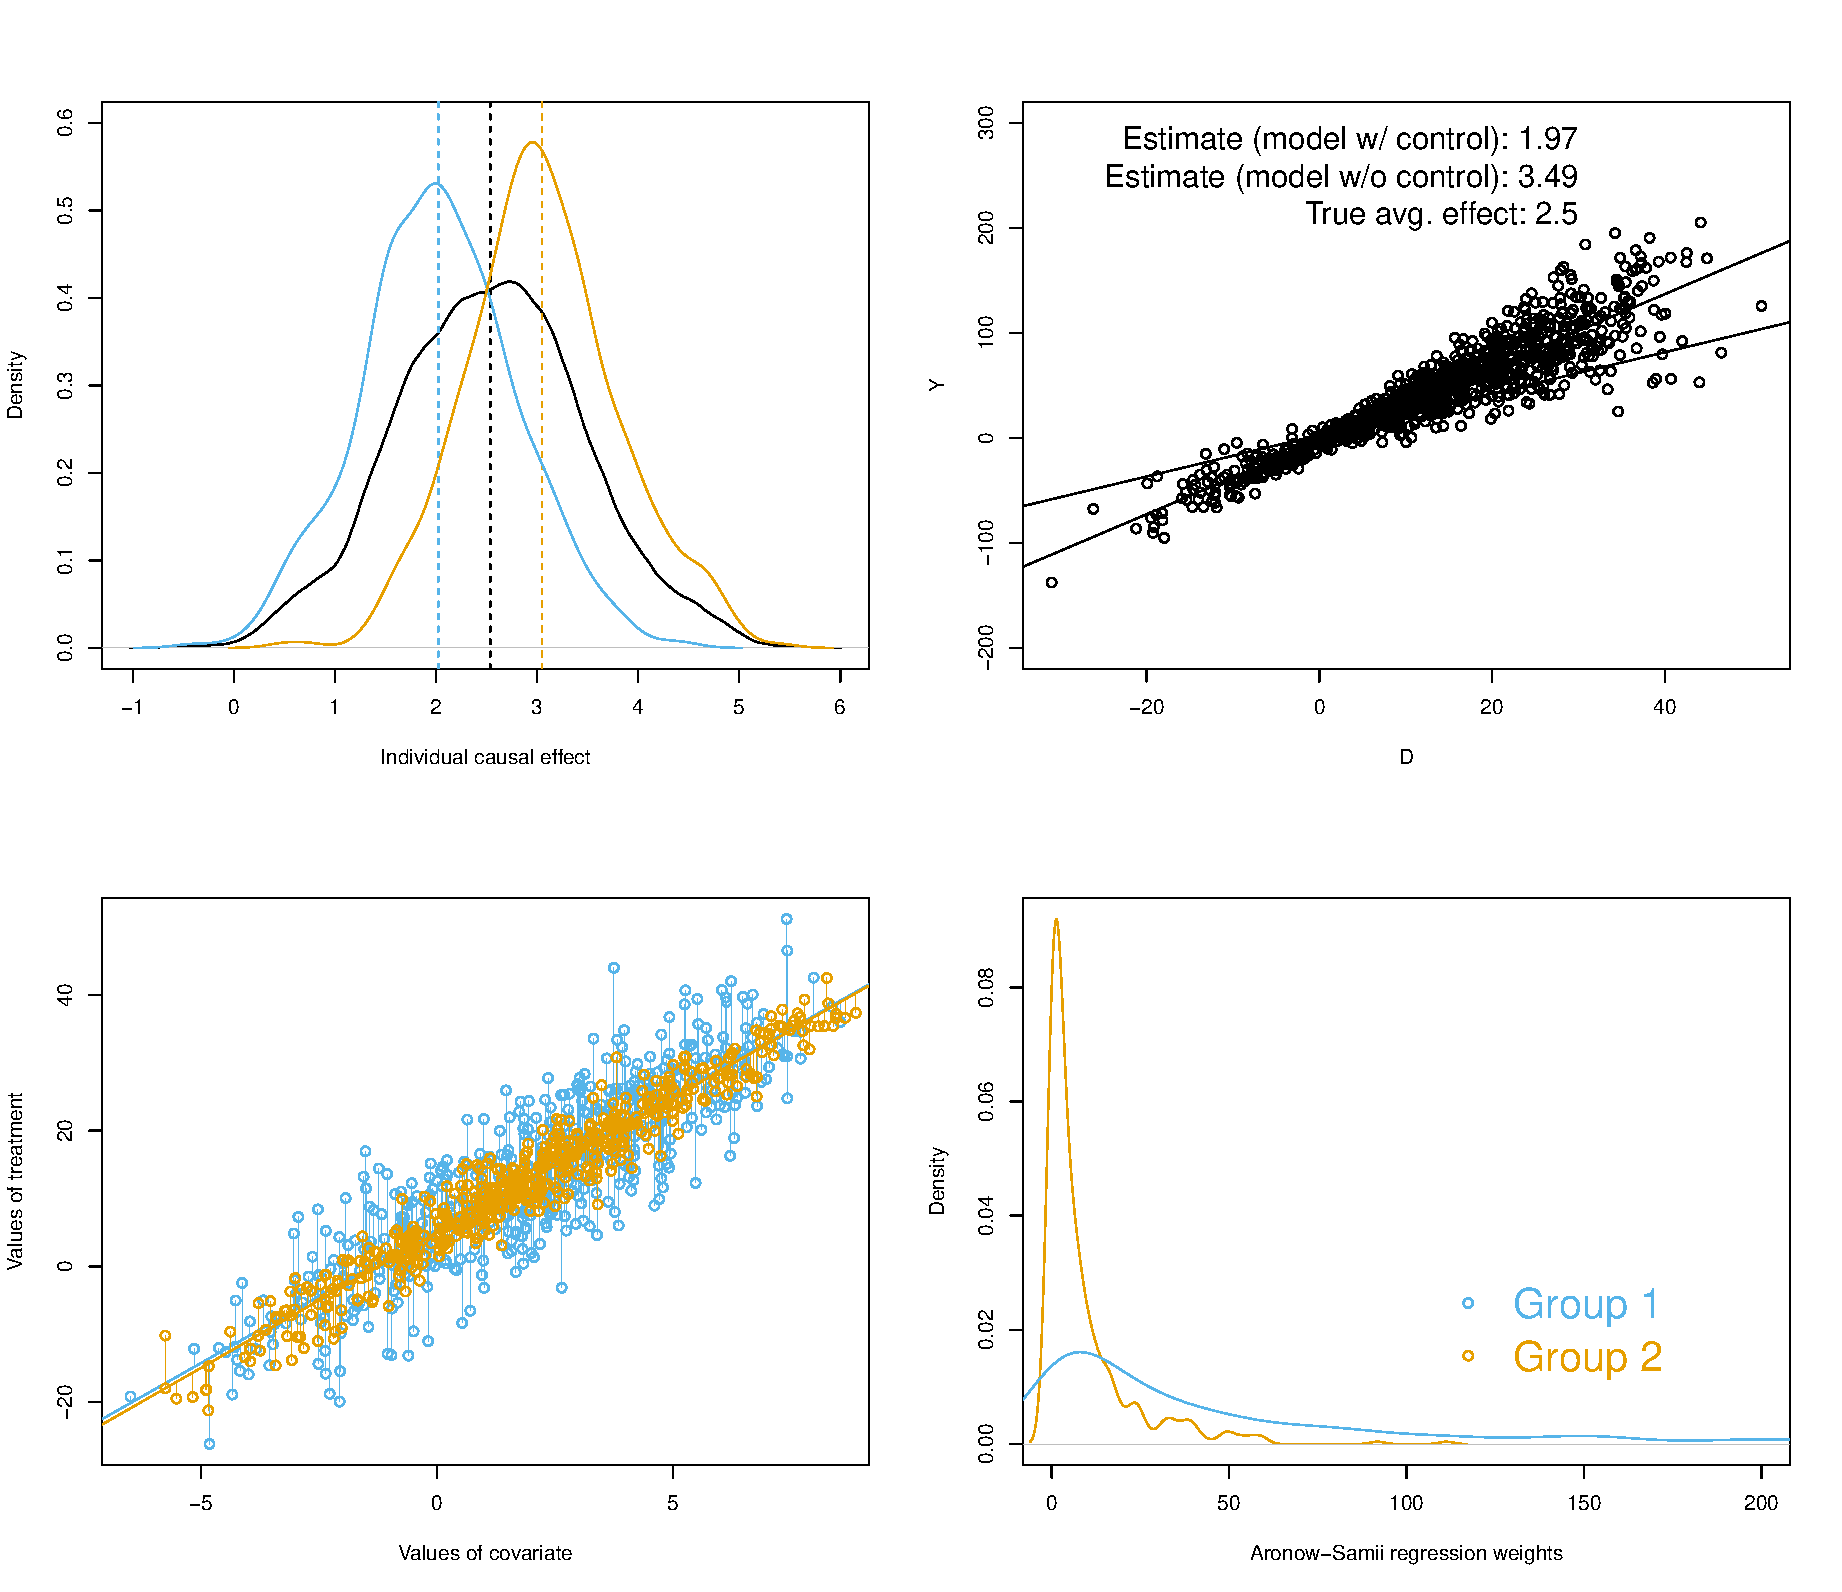
\includegraphics[width=\linewidth]{../plots/fig_1_a.pdf}
  \caption{\emph{There are two equally-sized groups of units in the sample, denoted blue and orange. We aim to recover the average causal effect, which averages over the individual causal effects in the entire sample. The top-left panel depicts the distribution of true individual causal effects in the sample (in black) and within each group; vertical lines show the true average causal effects in the population and within each group. The top-right panel shows the results of running an OLS regression controlling for X. Slopes are shown for models with and without controls. The estimate from the model with controls is less accurate than the estimate from the model without controls, even though we are controlling for a confounder. Notice that the estimate from the model with controls is closer to the average causal effect of individuals in group one than the average causal effect in the sample. The bottom-left panel shows the relationship between the treatment and the covariate for both groups. For units in group one, the covariate is a less precise predictor of treatment; the blue points fit the regression of treatment on the covariate less tightly. The bottom-right panel shows that, as a result, the Aronow-Samii regression-weights are much larger for group one. The larger group-one weights help explain why the estimates in the top-right panel are better approximations to the average causal effect in group one than in the sample as a whole.}}
  \label{fig_1_a}
\end{figure}

To illustrate the problems that may arise due to this heterogeneity, we divide our simulated sample into two equally sized groups, group one and group two. For both groups, treatment is a linear combination of the covariate plus some mean-zero noise. Causal effects are locally linear, meaning that, for each member of the sample, the effect of treatment on outcome is linear. Two characteristics, illustrated in the top- and bottom-left panels of Figure \ref{fig_1_a}, respectively, distinguish units in group one from group two. First, the average causal effect in group one is smaller in group one. Second, the covariate X is less prognostic of treatment in group one---knowing the covariate value for a unit in group one gives us less information about the treatment value than knowing the covariate value in group two.

Our target quantity, the average causal effect, gives equal weight to each of the individual causal effects across both groups. Yet when we regress the outcome on treatment and the covariate, we get estimates that are too small; in fact, they are much closer to the average causal effect in group one. This is true even though all the assumptions necessary for causal identification have been met and both treatment as well as outcome are simple linear functions of the covariate. What went wrong?

\citet{aronowsamii2016} derive a representation of the OLS estimator that helps answer this question. They show that, under the assumptions we have already specified, our estimated treatment effect, $\hat \beta_1$, converges in probability to the following quantity,

$$\hat \beta_1 \overset{plim}{\to} \frac{\mathbb{E}[w_i\tau_i]}{\mathbb{E}[w_i]} $$

where $w_i$ are given by the squared difference between the actual value that treatment takes on and the expected treatment value conditional on covariates.

$$w_i = (D_i - \mathbb{E}[D_i|X_i])^2$$

Within each covariate strata $X_i$, the expected value of the weights is equal to the conditional variance of our treatment given the covariate(s), $\mathbb{E}[D|X]$. The important takeaway is that when there is heterogeneity, OLS estimates variance-weighted average treatment effects---and always puts more weight on covariate strata where covariates do a poor job of explaining treatment assignment.

This dynamic is clearly at work in our toy example. Consider the bottom two panels of Figure \ref{fig_1_a}. The left panel shows that the covariate does a better job predicting the treatment in group two than in group one. The panel plots the relationship between treatment and covariates for each group. The units in group one and two are both just linear functions of covariate values, but this function is noisier and provides less information about treatment assignment in group one vs. group two, which is why the units in group one do not cleave to the regression line as closely as the units in group two. This discrepancy is reflected in the estimated Aronow-Samii weights. As shown in the right panel, the distribution of weights has a much fatter tail in group two, which makes sense in light of the covariate's reduced predictive power in group two.

The toy example is meant to illustrate that heterogeneity can bias OLS estimates even when the statistical model is correctly specified. Bias can arise purely from differences in how well covariates predict treatment across groups. A simple diagnostic in this case is to estimate the Aronow-Samii weights and plot the distribution of weights to see if there are any extreme weights, as in the lower-right panel of figure \ref{fig_1_a}. I provide an R script that takes the output from the regression model used to estimate the treatment effect and calculates the weights. The script works with several of the most popular R packages for estimating linear models.\footnote{The weights can be estimated by squaring the residuals from a regression of treatment on controls. The package can take as inputs \texttt{fixest}, \texttt{lm}, and \texttt{estimatr} model objects.}

\section{Sensitivity Analysis}

\citet{cinellihazlett2020} propose a procedure that probes the sensitivity of causal inferences made under the assumption of selection-on-observables. Their method allows analysts to evaluate how sensitive causal inferences are to confounders, or sets of confounders, with different levels of explanatory power.

In their set-up, the inferential danger posed by various potential confounders is exclusively determined by three quantities: how much variation treatment is uniquely explained by the potential confounder(s) after partialling out observed covariates, how much variation in the outcome is uniquely explained by the confounder(s) after partialling out both treatment and covariates, and how much variation in the outcome is uniquely explained by treatment after partialling out covariates. By considering the hypothetical values that the first two quantities---those that depend on the unobserved confounder---take in combination with the observed association of treatment and outcome, the analyst can construct tests to evaluate how severe confounding would have to be to eliminate a causal relationship. I examine the details of their proposal in detail below. After introducing the traditional omitted variable bias decomposition, I contrast it with Cinelli and Hazlett's. I then outline the key sensitivity parameters that can be derived from their framework.

\subsection{Classic omitted variable bias}

Traditionally, thinking about unobserved confounding has been guided by the formula for omitted variable bias (OVB). Cinelli and Hazlett's proposal is essentially a reformulation and extension of this simple result. Consider the following situation. We would like to estimate a simple model of the following form:

$$Y = \hat \tau D_i + \underbrace{\pmb{X}_i\hat \beta}_{Observed} + \underbrace{\hat \gamma Z}_{Unobserved} + \epsilon_{full}$$

Here, $\hat \tau$ is a consistent estimator of $D$'s effect on some outcome $Y$. But we only observe covariates in $X$, not $Z$. Hence, we can only estimate the following restricted regression which includes only observed variables:

$$Y = \hat \tau_{res}D_i + \pmb{X}_i\hat \beta_{res} + \epsilon_{res}$$
We know from Frisch-Waugh-Lovell that when there are two (or two sets) of regressors $D$ and $X$, we can recover $\hat \tau_{res}$, the coefficient on one regressor, through a residuals-on-residuals regression. We regress the residuals of a regression of $D$ on $X$ ($e^T_{D\sim X}$) on the residuals of a regression of $Y$ on $X$ ($e_{y\sim X}$).

$$\hat \tau_{res}= (e^T_{D\sim X}e_{D \sim X})^{-1}(e^T_{D \sim X}e_{y\sim X})$$
We can also think about this as a regression of Y on D where we have removed,  or "partialled out", the components of both that are linearly explained by $X$.

We can also write the coefficient from this regression in the following way:

$$\hat \tau_{res} = \frac{Cov[D^{\perp X},y^{\perp X}]}{V[D^{\perp X}]}$$
Expanding,
$$\hat \tau_{res}= \hat \tau + \frac{Cov[D^{\perp X},\gamma Z^{\perp X}]}{V[D^{\perp X}]} = \hat \tau + \hat \gamma \hat \delta$$
This is the classic OVB result. It says that the bias of our estimate $\tau_{res}$ is proportional to the product of two terms. The first term, $\hat \gamma$, is the estimated coefficient of the confounder in an unrestricted model where unobserved confounders are observed; the second, $\hat \delta$, is the imbalance of the unobserved confounder with respect to treatment within different covariate strata.

The practical use of the OVB result is limited. First, the result depends on the scale of the hypothetical unobserved confounder that we are accounting for. If we don't have a specific confounder with a known scale in mind, it is hard to make an argument about how robust the results truly are. Second, it is difficult to use the OVB result to understand the sensitivity of our result to a set of unobserved confounders, possibly acting jointly. Cinelli and Hazlett's proposal addresses both concerns.

\subsection{Omitted variable bias in terms of partial $R^2$}

Cinelli and Hazlett's key move is to express the bias term in the OVB result in terms of partial $R^2$. This formulation offers new insight into what is going on when unobserved confounders might bias our estimates. The absolute value of the bias term is rewritten in the below formula.

$$|bias| = \hat \delta \hat \gamma = se(\hat \tau_{res})\sqrt{\frac{R^2_{Y\sim Z|D,X}R^2_{D\sim Z|X}}{1-R^2_{D\sim Z|X}}df}$$
Where $se(\hat \tau_{res})$ is our estimate from the restricted model excluding the omitted variable and $df$ the degrees of freedom from the same model. The $R^2$ values can be interpreted as follows: $R^2_{Y\sim Z|D,X}$, for example, is the partial proportion of variance in the outcome explained by the unobserved confounder after partialling out the treatment and observed covariates. While this formulation is still a little opaque (to me, at least), it does yield a basic insight. The first is the asymmetry between the two quantitites in the second term. While the biasing effect of $R^2_{Y\sim Z|D,X}$ is bounded (since it can only go up to one), the biasing effect of $R^2_{D\sim Z|X}$ is not.

The real payoff of the partial $R^2$ formulation comes when we consider the absolute value of the bias as a proportion of point estimate:

$$|bias/\hat \tau_{res}|= \frac{|\overbrace{R^2_{Y \sim Z|D,X} \times \frac{R^2_{D \sim Z|X}}{1-R^2_{D \sim Z|X}}|}^{\text{Bias factor}} }{\underbrace{\frac{R^2_{Y \sim D|X}}{1 - R^2_{Y \sim D|X}}}_{\text{f(Variation in outcome explained solely by treatment)}}}$$
Note the key difference between the numerator and denominator in this expression. All terms in the numerator are functions of the observed data and unobserved confounder. The denominator is fully determined by an observed quantity. This formulation is nice because we can make precise some sort-of-obvious intuitions about omitted variable bias.

First, consider the case where we hold fixed the severity of unobserved confounding, as expressed by the $R^2$ values in the numerator. In this case, the proportion of bias relative to our estimate is solely determined by the size of the denominator. When the amount of variation in the outcome uniquely explained by the treatment is large, bias as a proportion of our point estimate will go down.

Second, consider the extreme case where a confounder explains all of the variation in treatment after partialling out treatment and observed covariates. In such a case, the first term in the numerator goes to one, and we are left with a simple ratio. This formulation thus allows for the relatively simple construction of a "worst-case" sensitivity analysis.

\subsection{Sensitivity quantities}

I now consider two simple quantites that Cinelli and Hazlett suggest analysts report. Substantively, I show how these quantities can provide insight into the robustness of the estimates from a recently published article \citet{hankinson2018}.

\subsection{Replication study}

In a survey of voters sampled from areas where housing policy is locally determined, \citet{hankinson2018} asks respondents about their preferences for policies that increase housing supply. He evaluates support for two potential policies: a policy designed to increase supply by ten perecent, and a ban on new housing development.

Figure \ref{hankinson1} plots the results from a series of OLS regressions. The regressions estimate the expected support for both policies conditional on homeownership, after stratifying by covariates. In expectation, homeowners are nearly ten percent more likely to support a ban on neighbourhood development than renters and twenty percent less likely to support a ten percent increase in housing supply. Results are qualitatively similar when support for policies is measured on a seven-point likert scale.

\begin{figure}
  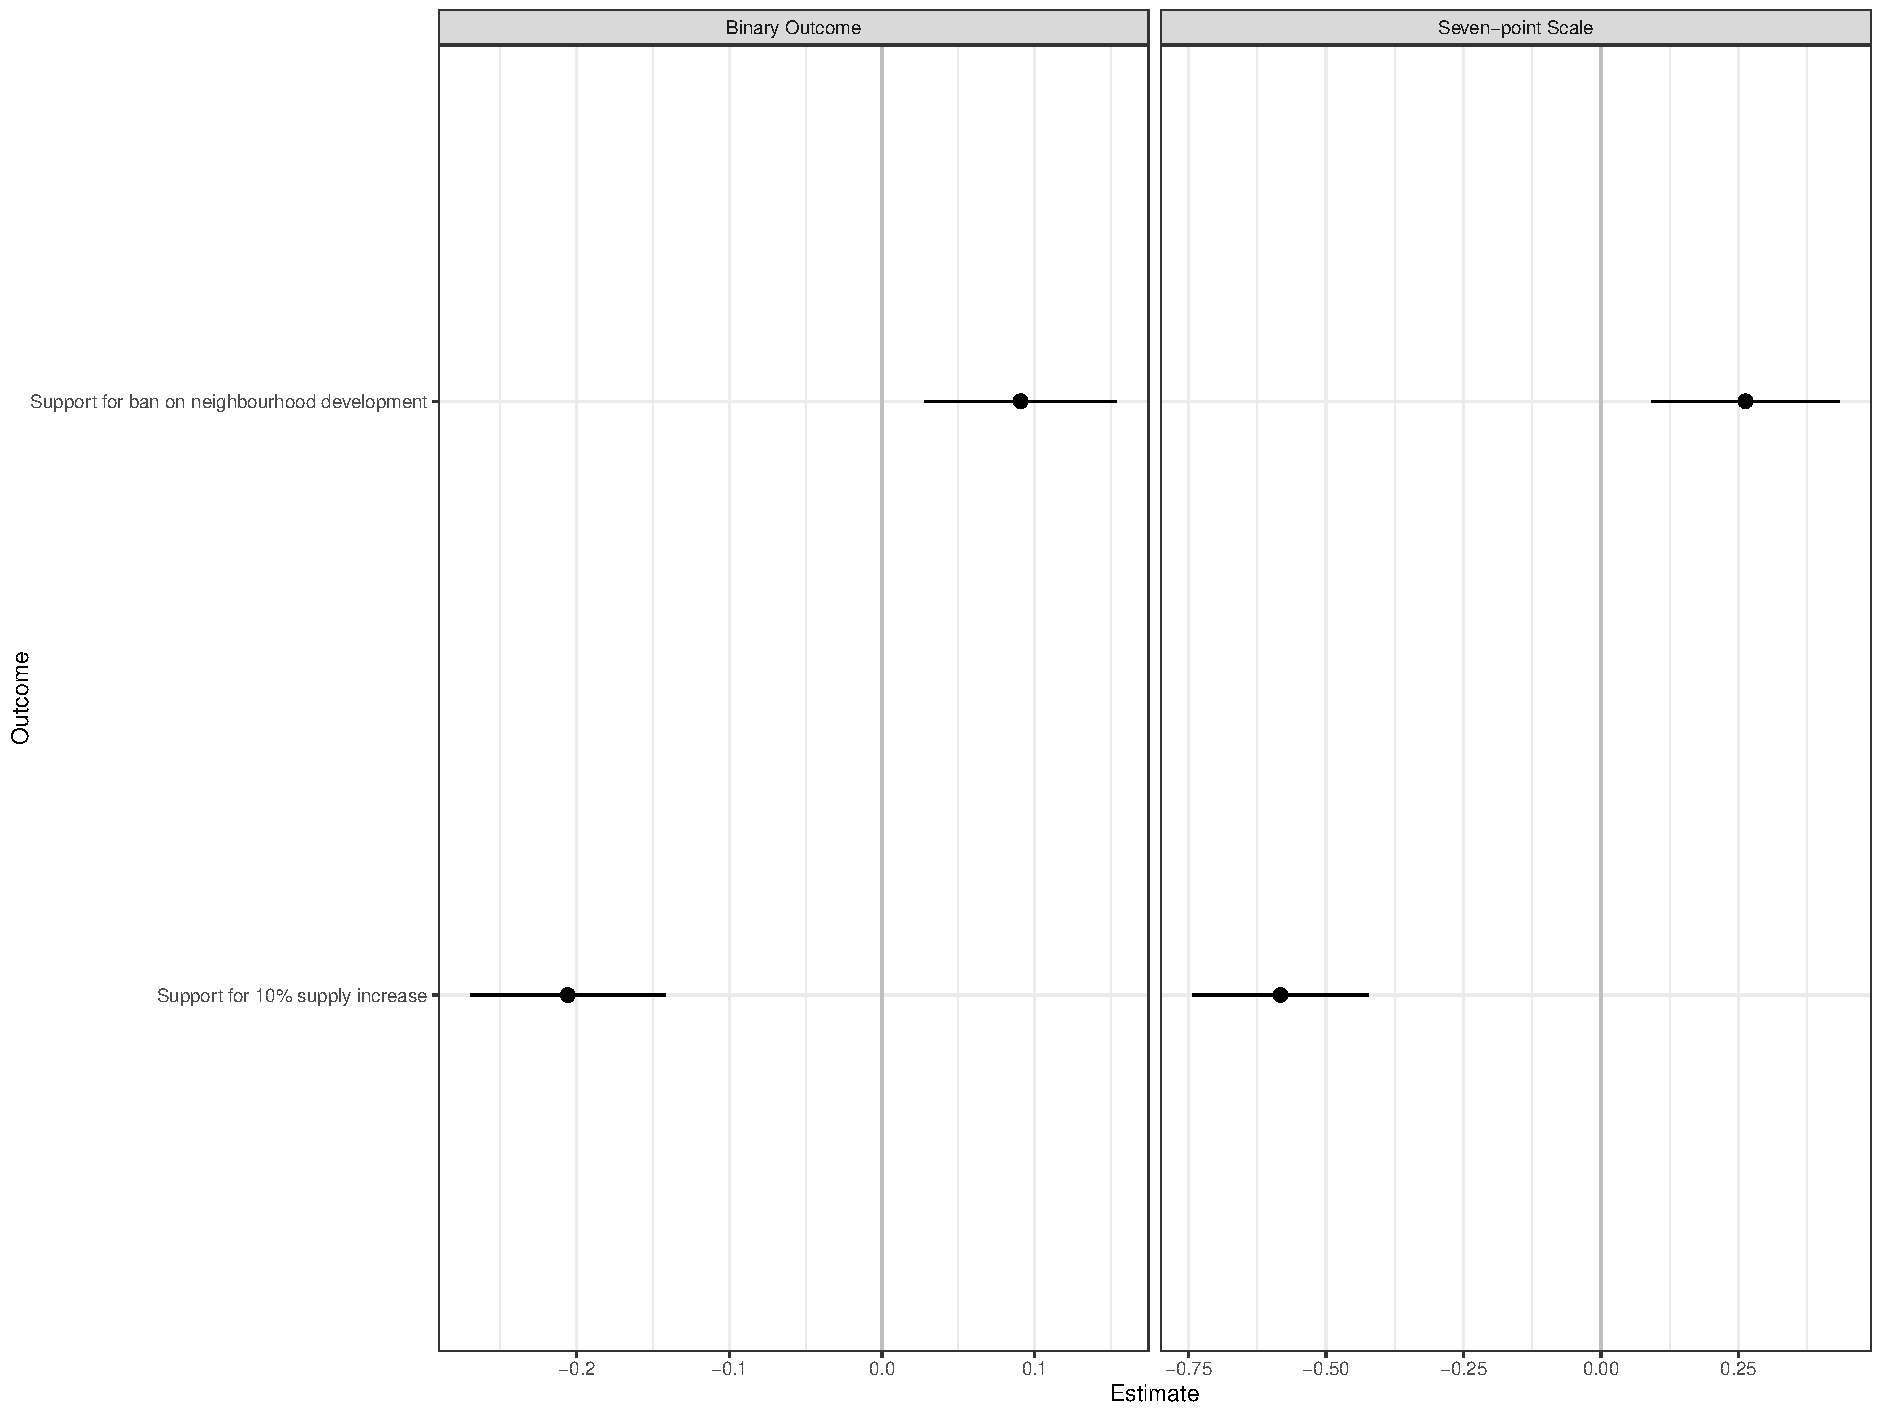
\includegraphics[width=\linewidth]{../plots/hankinson1.pdf}
  \caption{\emph{The plot reports point estimates from OLS regressions with respondent homeownership as treatment and support for housing policies as response. The left panel plots answers on a binary 'support'/'do not support' scale, the right panel plots answers on a seven-point likert scale. Respondents are sampled from a set of zip codes where housing policy is determined at the municipal level and the housing policies are suggested as hypothetical municipal ballot measures.}}
  \label{hankinson1}
\end{figure}


\subsection{Worst case sensitivity analysis}

Say we assume all variation in outcome that isn't uniquely explained by treatment after partialling out observed covariates X is explained by a confounder, implying that $R^2_{Y\sim Z|D,X}=1$. \emph{How strong would the association between treatment and confounder after partialing out observed covariates need to be to bring the coefficient down to $<0$?}

The sensitivity parameter that answers this question is simply the quantity $R^2_{Y\sim D|X}$, the proportion of outcome variation explained by the treatment after partialling out $X$. To consider why this is the case, we rewrite the formula for bias as a proportion of the treatment effect, taking into account that we have assumed $R^2_{Y\sim Z|D,X}=1$.

$$|bias/\hat \tau_{res}|= \frac{|\overbrace{1 \times \frac{R^2_{D \sim Z|X}}{1-R^2_{D \sim Z|X}}|}^{\text{Bias factor}} }{\underbrace{\frac{R^2_{Y \sim D|X}}{1 - R^2_{Y \sim D|X}}}_{\text{Variation in outcome explained solely by treatment}}}$$
When the above expression, the relative bias, is equal to 1, the bias is large enough to push our coefficient down to zero. To make it one, the two remaining $R^2$ terms need to balance each other out. That just means that the partial $R^2$ of the treatment and confounder after partialling out $X$ has to be equal to the partial $R^2$ of the treatment and outcome after partialling out $X$.

Figure \ref{hankinson2} shows the results of a sensitivity analysis under these assumptions. Keeping the confounder-outcome relationship fixed, we observe that the bias in our estimates is large enough to push coefficients under zero even if the confounder explains less than ten percent of the residual variation in treatment after partialling out covariates. In terms of Hankinson's estimates: if an unobserved confounder, say aesthetic preferences for single-family housing, explains half the residual variation in housing policy preferences, then figure three shows how much of the residual variation in homeownership aesthetic preferences the confounder would have to explain to bias the point estimate to zero. Here, that number is less than ten percent.

\begin{figure}
  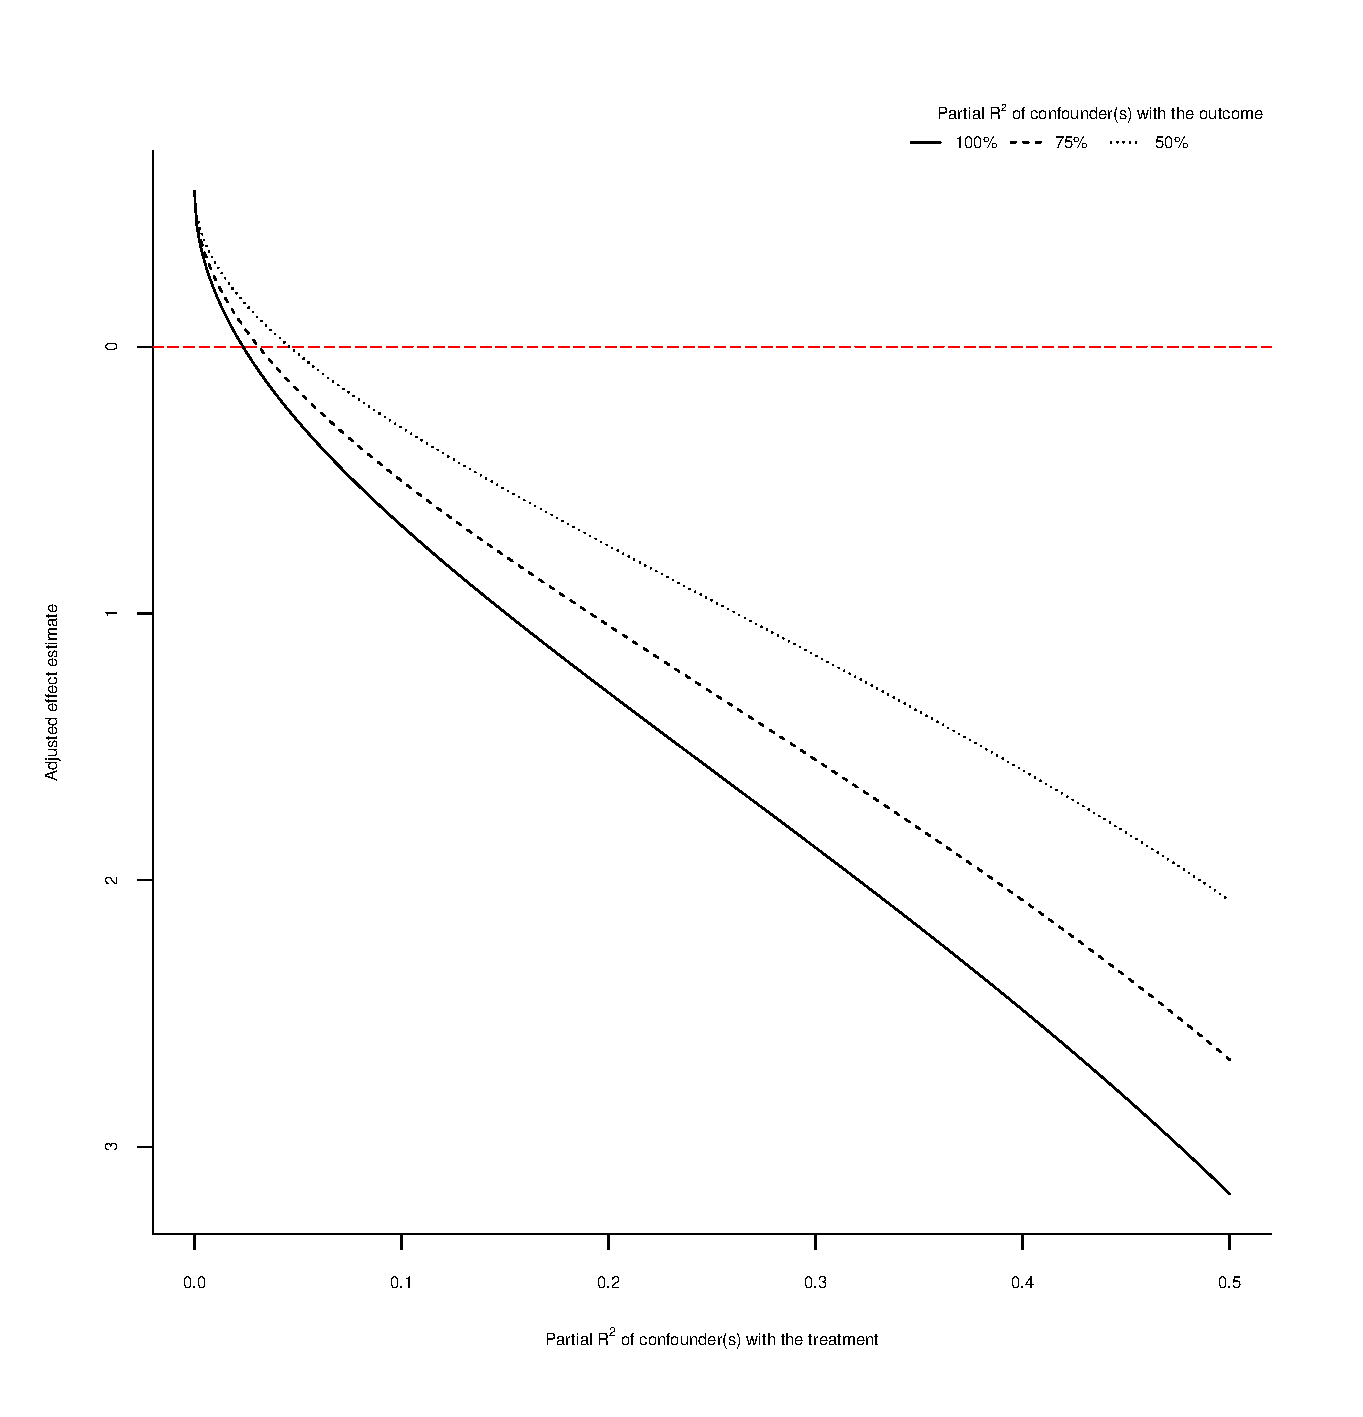
\includegraphics[width=\linewidth]{../plots/hankinson2.pdf}
  \caption{\emph{The plot reports estimates of the effect of homeownership on support for policy increasing housing supply after adjusted for unobserved confounding of varying severity. The lines labeled 50, 75, and 80 percent denote assumptions about how much variation in the outcome is uniquely explained by a hypothetical unobserved confounder after partialling out covariates and treatment. The plot depicts how severely estimates are biased as the proportion of variance in treatment explained by the unobserved confounder increases.}}
  \label{hankinson2}
\end{figure}



\subsection{Robustness values}

The main quantity that Cinelli and Hazlett suggest analysts report is the robustness value (r-value). The  r-value allows analysts to evaluate the sensitivity of their results under the assumption that a confounder is equally associated with treatment after partialling out covariates and with the outcome after partialling out treatment and covariates. It then asks: \emph{how strong would the confounder-treatment and confounder-outcome association need to be to push the estimate down by a certain proportion of the estimate?} More precisely, how strong would the association need to be to reduce our estimate by $q100$ \%? The r-value is that answer to this question and is calculated as such:

$$RV(q) = \frac{1}{2}\(\sqrt((qf^4_{Y\sim D|X} + 4qf^2_{Y\sim D|X})-qf^2_{Y\sim D|X})\)$$

where $f_{Y\sim D|X}$ is the cohen's $f$ of treatment and outcome after partialling out covariates (which is an increasing function of the partial $R^2$ discussed above). For any $q$, the r-value tells us how strong the confounder-outcome and confounder-treatment associations would need to be after partialling out in order to reduce the magnitude of our effect by $q100$ \%. When $q=1$, the default, it asks how strong the association would need to be to push the effect size to zero.

\begin{figure}
  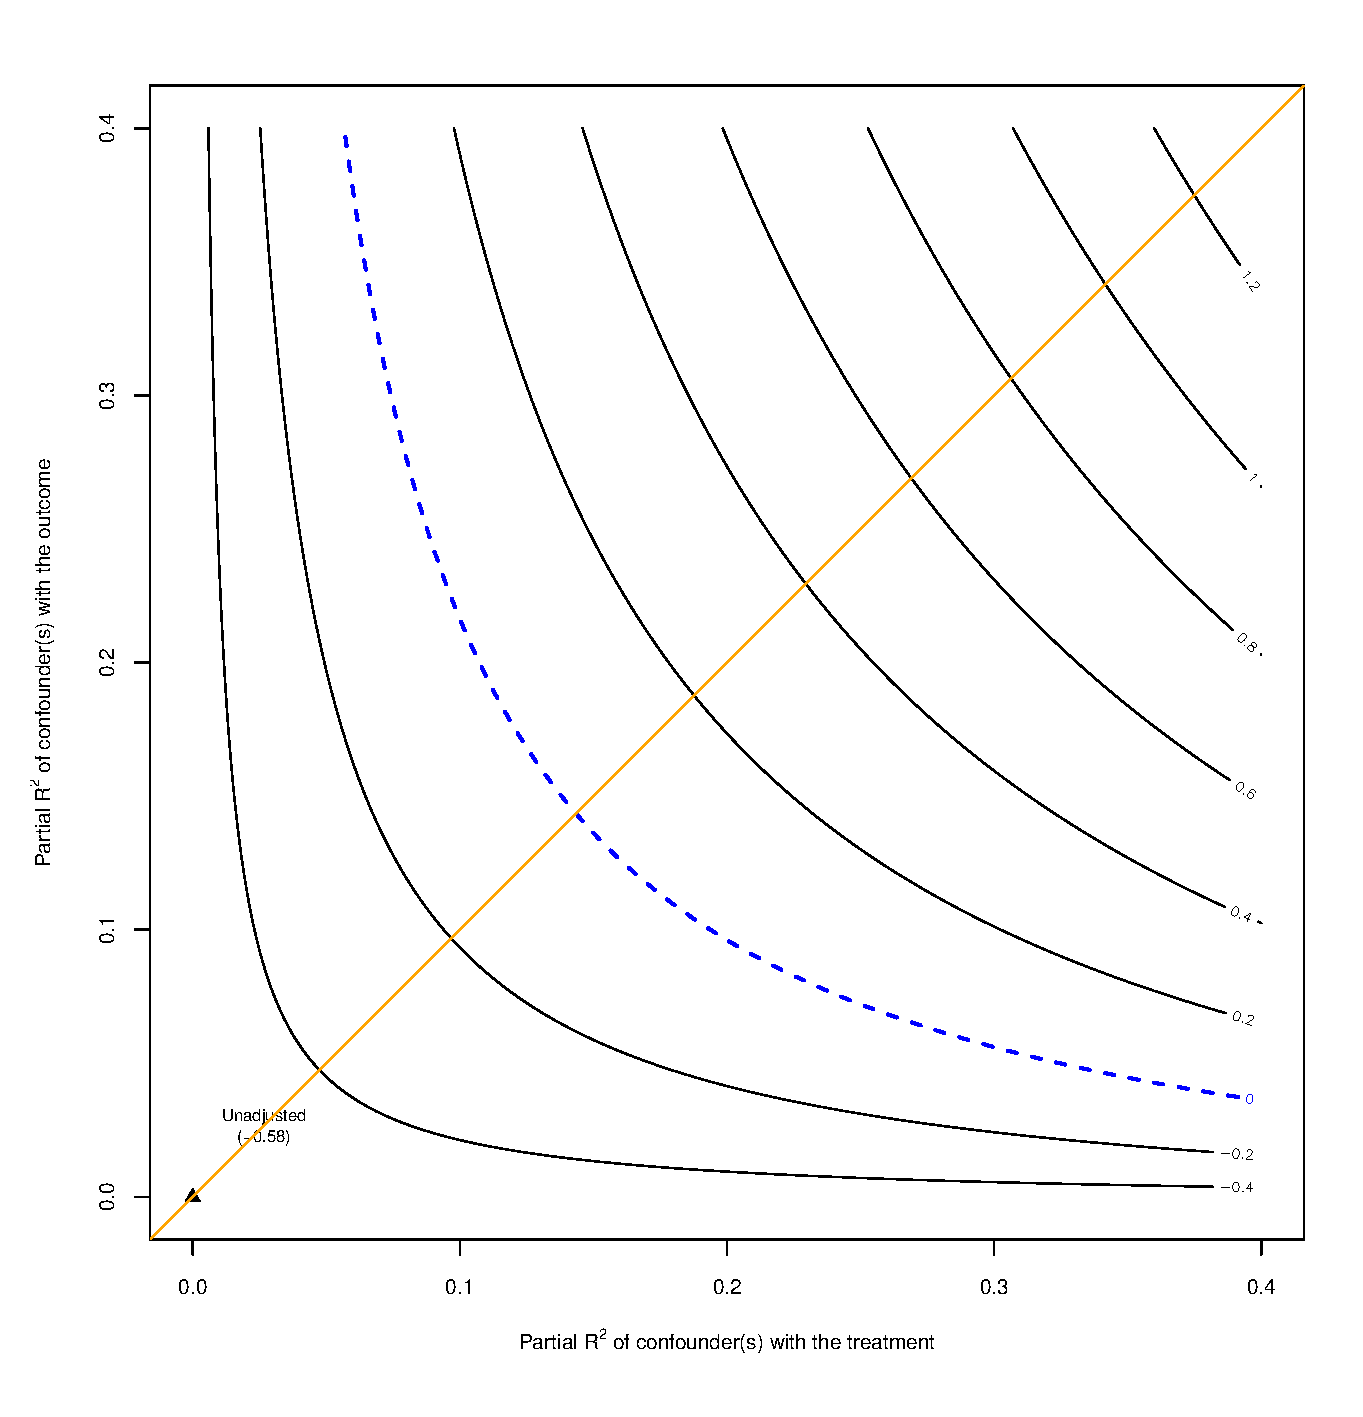
\includegraphics[width=\linewidth]{../plots/hankinson3.pdf}
  \caption{\emph{The plot reports the biasing effects of different combinations of partial $R^2$ values on the point estimates reported in the bottom right panel of figure 1. Each point on the plot represents a potential confounder of different strength. X-axis values represent the amount of residual variation in homeownership that a potential confounder explains after partialling out covariates. Y-axis values represent the amount of residual variation in preferences for expanding the housing supply that the confounder explains after partialling out covariates and homeownership. The dashed blue line partitions the plot into a region where bias from potential confounders reverses the sign of the estimate, and a region where the sign of the estimate remains the same. Any potential confounders located in the region to the right of the blue line are strong enough to bias the estimated negative effect up to a value greater than zero. The orange line depicts the biasing effects of potential confounders that have the same partial $R^2$ with both treatment and outcome. The robustness value that Cinelli and Hazlett suggest analysts report is simply the partial $R^2$ of such a confounder that is sufficient to bias estimates to zero. Graphically, the robustness value is the point where the orange and blue lines cross.}}
  \label{hankinson3}
\end{figure}



Consider again the estimates from Hankinson evaluated in the previous section. We calculate that unobserved confounders that uniquely explain 14\% or more of the residual variation in both home-ownership and opinions about building affordable housing are enough to bring the estimated effect of home-ownership on preferences for expanding the housing supply to zero. Figure \ref{hankinson3} provides graphical intuition for the r-value.

\begin{figure}
  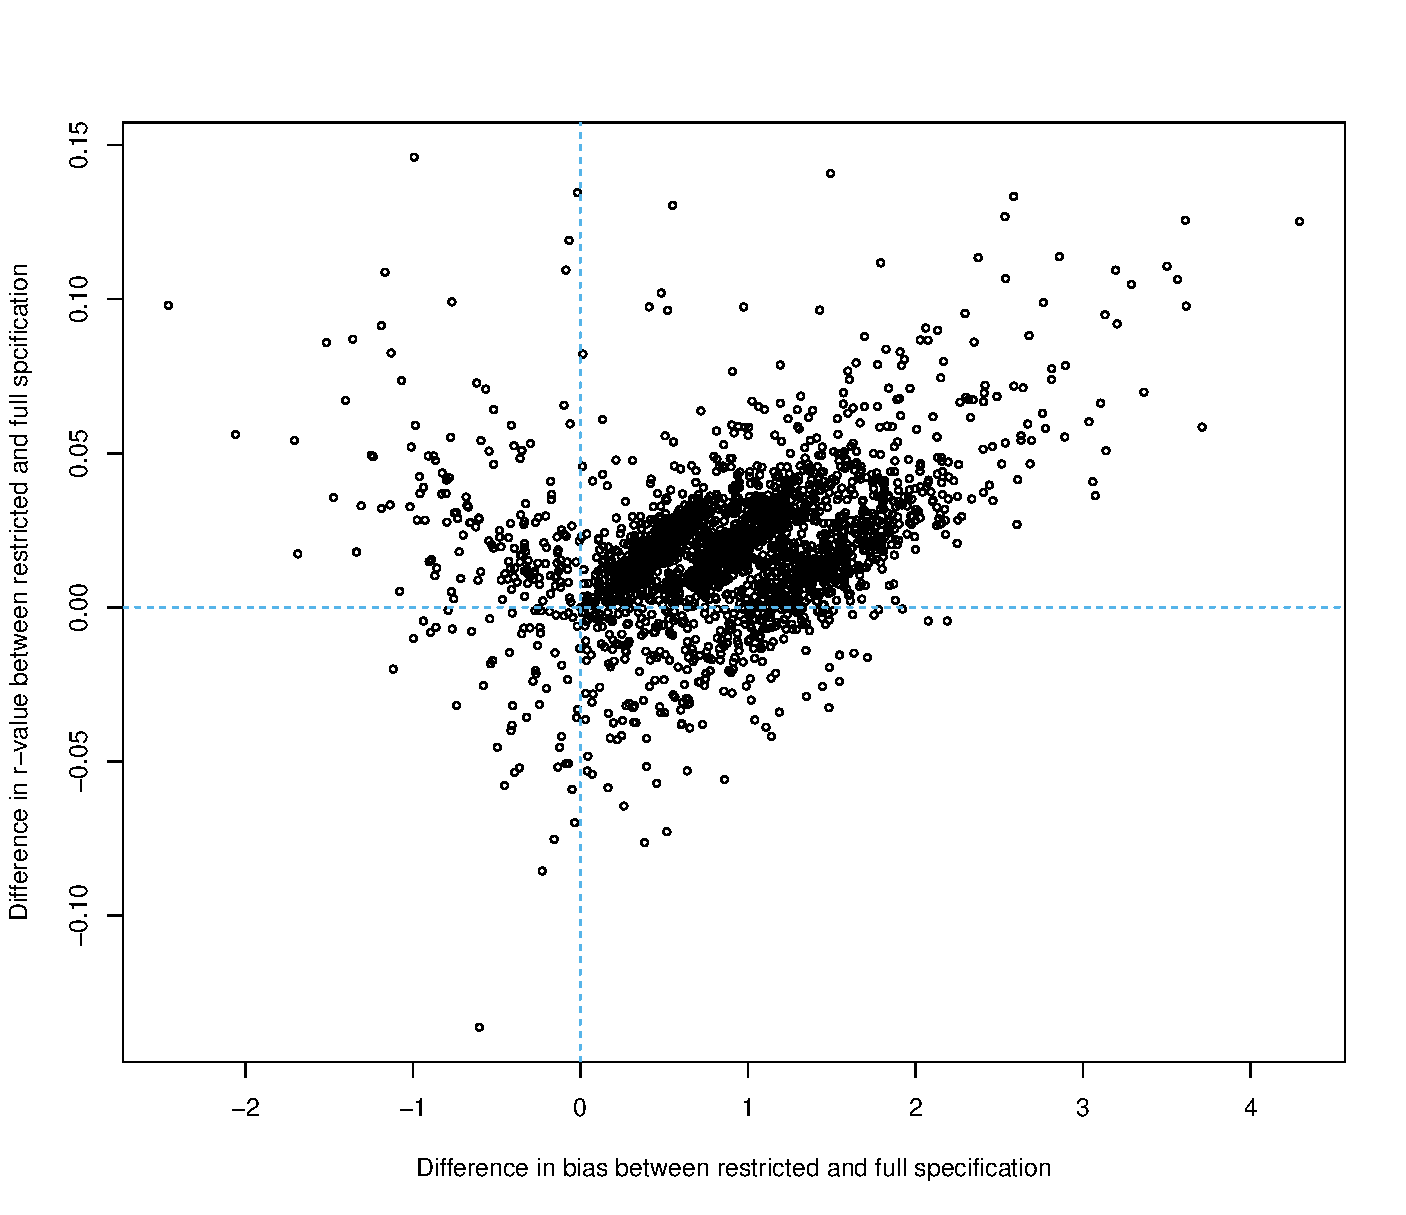
\includegraphics[width=\linewidth]{../plots/cov_prob.pdf}
  \caption{\emph{Data is simulated from a similar data-generating process as used during the simulations for binary treatments, but with varying levels of confounding. Each point on the plot is calculated using regressions from one simulated data set. The y-axis plots the estimated bias of a restricted model including some, but not all, confounders minus the bias of a full model including all confounders. It can be thought as measuring the additional bias incurred by not including all confounders. Points on the x-axis also plot a comparison between restricted and full models, this time between the robustness value of the restricted and full models. Points in the upper-right quadrants represent data for which the restricted model is more biased yet also has a higher robustness value. Most of the points are located in this quadrant, indicating that it is common for more biased estimators to produce estimates with a higher robustness value.}}
  \label{cov_prob}
\end{figure}

While the robustness value clearly has benefits, some care must be taken in interpreting it correctly. Comparing r-values from different treatments or different specifications is unlikely to be informative as specifications with higher r-values do not constitute stronger evidence. The reason is intuitive and illustrated by figure \ref{cov_prob}. It shows the results from simulations similar to those previously presented for binary treatments (the only difference is in the parametrization of some of the distributions, not in the functional forms). Once again, researchers only observe a transformed and coarsened version of the confounding covariates. The figure compares the estimated bias (the difference between estimated and true average causal effect) of restricted regressions that only include two of the three confounding variables to the bias of full regressions which include all unmeasured confounders. The y-axis plots the additional bias incurred by estimating the restricted instead of the full model; the x-axis plots the difference in  r-values between the two models. The clear takeaway is that, in these simulations, more biased specifications that include fewer confounders usually have larger r-values.

This seems strange: it is intuitive that studies which measure more confounding variables are more ``robust'' in some general sense, not less robust as these simulation results would seem to imply. The fact that this intuition is not borne out helps clarify what sensitivity parameters like the r-value can and cannot do. What could be going on in this case is that the ability of an unobserved confounder at any given level of confounder-outcome association to bias estimates increases as the treatment explains less variation in the outcome after partialling out confounders. When we include additional confounders that strongly predict the outcome, as we do in the full models, the treatment explains less variation in the outcome after partialling out confounders. The r-value reflects the fact that there is more variation in the outcome that the treatment does not explain. That the inclusion of such confounders might reduce the r-value does not in any way indicate that the r-value is not a useful measure of sensitivity. Instead, it is a reminder that sensitivity parameters can only be evaluated within the context of the model they are calculated from. When we have taken greater care to observe all plausible confounders, as we did in the full model, relatively low r-values may constitute good evidence that the results are robust to unobserved confounding; when we have taken less care to observe confounders, as in the restricted model, relatively high r-values may not offer sufficient reassurance that results are robust. Comparing r-values across these specifications without contextual knowledge about how well they do in picking up on unobserved confounding will lead us astray.

\section{Conclusion}

The purpose of this review was to highlight tools for diagnosing and dealing with violations of key assumptions in the OLS framework for estimating average causal effects. As I keep on working on this piece, I want to add several things. First, I am working on R code that automatically produces helpful visualizations of the Aronow-Samii weights from model objects. I am currently playing around with various options as I work on integrating the Hankinson replication into the section about weighting. Second, I also want to discuss methods for sensitivity analysis that propose sensitivity parameters based on the proportion of units that are unconfounded/confounded \citep{bonvinikennedy2021}. Finally, I want to link the results on sensitivity analysis with those concerning non-parametric bounds.

\bibliography{/users/oliverlang/bibliography1}
\end{document}


regime shocks -> lower “adaptive capabilities”

farmers get quotas: sell back to state at fixed prices
amentities free for forced laborers.
individual pickers get quotas: norm
